\section{Activation Caps Reduce Adam Loss Spikes}
\label{sec:vc-interventions}

Motivated by the large changes in outputs and hidden representations observed at loss peaks (Fig.~\ref{fig:trace-motion}), we test a training intervention that limits Adam updates when they induce large changes in neuronal responses. From Eq.~\eqref{eq:adam-update}, Adam proposes the parameter increment $\Delta\theta_t=-\eta_t d_t$. Let $\Delta\theta_{t,j}^{\ell}$ be the block of this increment for unit $j$ at site $\ell$. Each row of $H_t^\ell$ contains the inputs to the unit for one reference example or position.\footnote{Each row holds the values under a convolutional filter at one position or, in self-attention, the token representation used to compute its query, key, and value. For units with a bias, we include its update in the parameter block and append a column of ones to $H_t^\ell$.} Holding these inputs fixed, the root-mean-square (RMS) change in the unit's response is
\begin{equation}
 s_{t,j}^{\ell}=\frac{\|H_t^\ell\,\Delta\theta_{t,j}^{\ell}\|_2}{\sqrt n}.
 \label{eq:vc-score}
\end{equation}
When this displacement exceeds the site budget $\tau_\ell$, we scale down the unit's proposed increment according to
\begin{equation}
 \Delta\theta_{t,j}^{\ell,\mathrm{cap}}
 =\gamma_{t,j}^{\ell}\,\Delta\theta_{t,j}^{\ell},\qquad
 \gamma_{t,j}^{\ell}=\min\!\left(1,\frac{\tau_\ell}{s_{t,j}^{\ell}}\right).
 \label{eq:vc-cap}
\end{equation}
Since $\gamma_{t,j}^{\ell}\in[0,1]$, the cap can only reduce the magnitude of each unit's update, without reversing its direction. It is applied after Adam's moment estimates are updated, leaving them unaffected. The constraint bounds only the unit's direct response change with fixed inputs, without accounting for changes propagated from earlier layers. We calibrate each site's budget $\tau_\ell$ using the 25th, 50th, or 75th percentile (q25, q50, or q75) of unit displacements pooled over the eight Adam updates preceding the intervention. We apply the cap to the MLP's two hidden linear maps, all ResNet convolutions, and the Transformer's query, key, value, and feed-forward projections.

\begin{figure*}[!t]
\centering
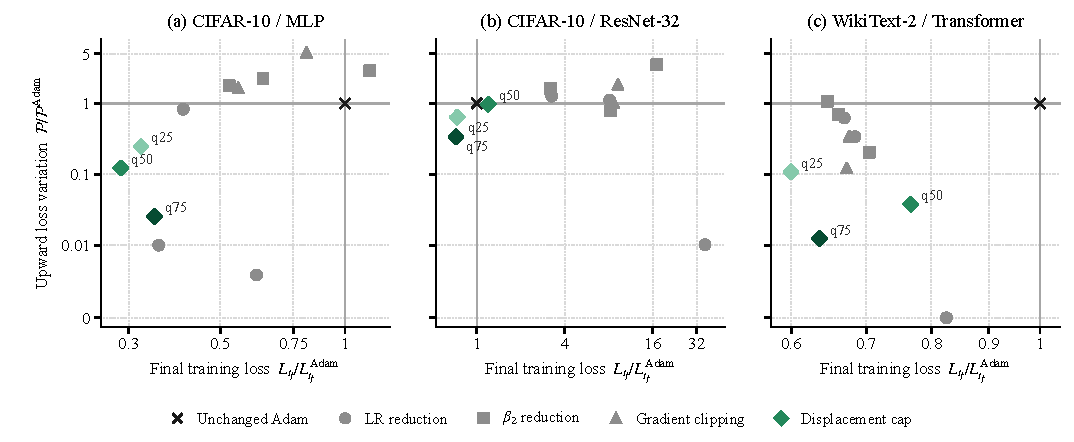
\includegraphics[width=\textwidth]{figures/24-main-intervention-tradeoff.pdf}
\caption{Final training loss and accumulated upward loss variation for 11 interventions, each expressed as a ratio to unchanged Adam for the same model. The solid lines intersect at the Adam baseline $(1,1)$. Points below and to its left improve both outcomes. Horizontal axes are logarithmic with model-specific ranges. The shared vertical axis is linear up to $0.005$ and logarithmic above it. Table~\ref{tab:vc-outcomes} reports the absolute values.}
\label{fig:vc-tradeoff}
\end{figure*}

To compare interventions, we resume training from identical parameters, Adam moments, and random states for the same number of full-batch updates. We evaluate the three activation caps against unchanged Adam, reduced learning rates, lower second-moment coefficients $\beta_2$~\cite{bai2026spikes}, and global gradient clipping~\cite{pascanu2013difficulty}. We measure optimization performance by final loss $L_{t_f}$ and mean loss $\bar L$, and quantify instability through cumulative upward loss variation $\mathcal P$
\begin{equation}
 \mathcal P=\sum_{t=t_0+1}^{t_f}\max(L_t-L_{t-1},0).
 \label{eq:vc-outcomes}
\end{equation}

\begin{table*}[!tp]
\caption{Absolute matched training outcomes. Lower is better. Bold marks each column minimum at full precision.}
\label{tab:vc-outcomes}
\centering\fontsize{8.5}{10.5}\selectfont
\setlength{\tabcolsep}{4pt}
\renewcommand{\arraystretch}{1.13}
\begin{tabular}{llrrrrrrrrr}
\toprule
 & & \multicolumn{3}{c}{CIFAR-10 / MLP} & \multicolumn{3}{c}{CIFAR-10 / ResNet-32} & \multicolumn{3}{c}{WikiText-2 / Transformer} \\
\cmidrule(lr){3-5}\cmidrule(lr){6-8}\cmidrule(lr){9-11}
Intervention & Parameter value & $10^3 L_{t_f}$ & $10^3\bar L$ & $10^3\mathcal P$ & $10^3 L_{t_f}$ & $10^3\bar L$ & $10^3\mathcal P$ & $10^3 L_{t_f}$ & $10^3\bar L$ & $10^3\mathcal P$ \\
\midrule
Adam & --- & 30.3 & 20.8 & 288.4 & 6.7 & 176.5 & 1314.9 & 917.8 & 849.6 & 5886.7 \\
\addlinespace[3pt]
\multirow{3}{*}{LR reduction} & $0.75\eta$ & 12.3 & 17.3 & 237.9 & 21.8 & 206.2 & 1662.6 & 614.0 & 824.3 & 3655.5 \\
 & $0.5\eta$ & 10.7 & 15.6 & 2.9 & 54.5 & 224.5 & 1460.9 & 627.7 & 753.1 & 2001.7 \\
 & $0.1\eta$ & 18.5 & 20.1 & \textbf{1.2} & 244.7 & 334.4 & \textbf{13.4} & 757.2 & 802.7 & \textbf{0.0} \\
\addlinespace[3pt]
\multirow{3}{*}{$\beta_2$ reduction} & 0.95 & 19.2 & 24.3 & 648.8 & 114.2 & 226.7 & 4606.1 & 593.0 & 759.0 & 6307.0 \\
 & 0.9 & 15.9 & 24.6 & 513.2 & 21.4 & 170.3 & 2147.5 & 606.7 & 706.5 & 4137.5 \\
 & 0.5 & 34.8 & 47.2 & 829.1 & 55.1 & 187.6 & 1028.9 & 646.2 & 767.8 & 1200.6 \\
\addlinespace[3pt]
\multirow{2}{*}{Gradient clipping} & 0.5 & 16.7 & 21.2 & 476.7 & 57.8 & 202.1 & 1348.5 & 617.0 & 698.5 & 723.3 \\
 & 1 & 24.4 & 30.8 & 1497.6 & 62.0 & 199.9 & 2441.0 & 620.1 & 717.3 & 2027.5 \\
\addlinespace[3pt]
\multirow{3}{*}{Displacement cap} & q25 & 9.7 & 14.4 & 71.2 & 4.9 & \textbf{138.4} & 840.3 & \textbf{550.5} & 692.7 & 638.0 \\
 & q50 & \textbf{8.7} & \textbf{14.1} & 35.3 & 8.0 & 159.9 & 1278.4 & 703.9 & \textbf{681.0} & 221.7 \\
 & q75 & 10.5 & 15.0 & 7.3 & \textbf{4.8} & 142.1 & 445.2 & 583.3 & 681.6 & 72.7 \\
\bottomrule
\end{tabular}
\end{table*}


\begin{figure*}[!tp]
\centering
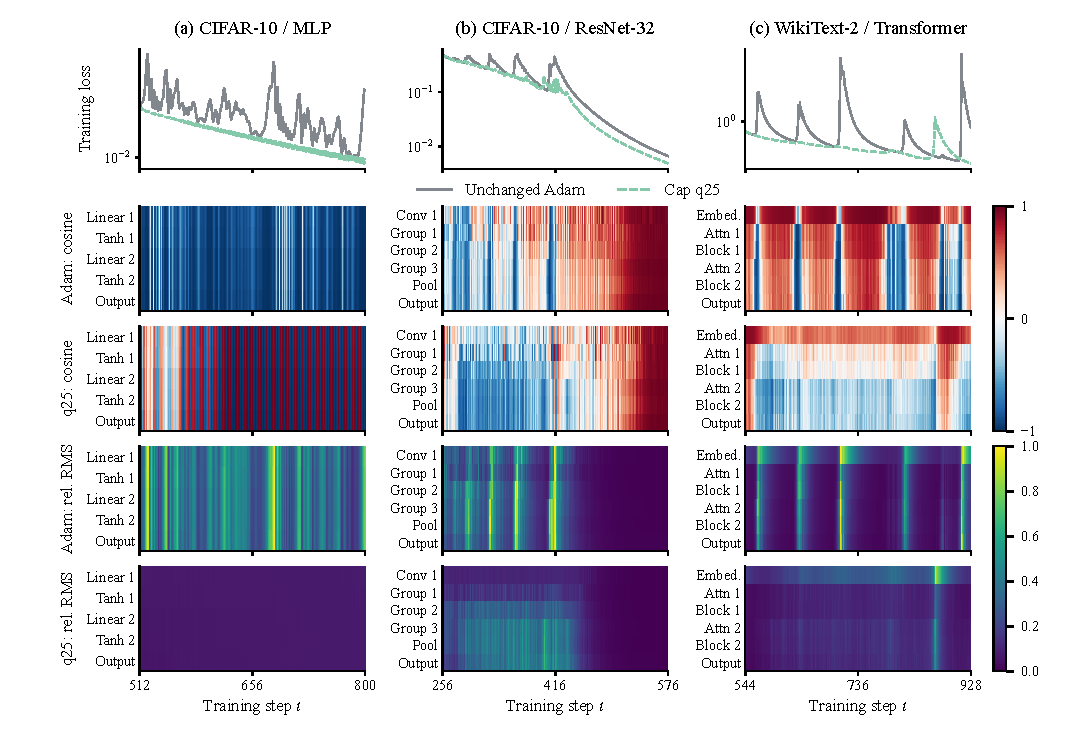
\includegraphics[width=.97\textwidth]{figures/25-main-q25-functional-motion.pdf}
\caption{Training loss and representation changes under unchanged Adam and the q25 activation cap. Top: training loss. Below: cosine between consecutive representation changes and RMS displacement at the measured sites, evaluated on the same reference inputs. For each site, RMS displacement is normalized by its maximum under unchanged Adam, allowing direct comparison between interventions.}
\label{fig:vc-motion}
\end{figure*}

All three activation caps reduced mean training loss and accumulated upward loss variation across all models (Table~\ref{tab:vc-outcomes}). Among the tested interventions, q50 achieved the lowest mean loss in the MLP and Transformer, while q25 performed best in ResNet. These results highlight a trade-off between suppressing loss spikes and reaching lower-loss solutions: reducing the learning rate can limit further optimization, whereas activation caps can improve both outcomes (Fig.~\ref{fig:vc-tradeoff}). For example, a tenfold learning-rate reduction in ResNet suppressed upward loss variation by 99\% but increased final loss from 0.0067 to 0.245. In contrast, q25 reduced final loss to 0.0049.

To examine the effect on network representations, Fig.~\ref{fig:vc-motion} compares q25 with unchanged Adam, as this setting improved all three training metrics across models. The largest RMS change in predictions decreased by 93\%, 33\%, and 45\% in the MLP, ResNet, and Transformer, respectively. Nevertheless, consecutive output changes remained negatively aligned on 50\%, 60\%, and 89\% of updates. Thus, activation caps substantially reduce the magnitude of functional changes without eliminating destructive oscilation, suggesting that controlling their amplitude can improve training without suppressing oscillatory dynamics entirely. Activation caps, however, introduce computational overhead by requiring estimates of each unit's response to the proposed update. Although preliminary, these findings point toward a broader research direction: can we develop training algorithms that regulate updates based on how they affect the network's learned representations, rather than solely on gradient or parameter magnitudes?


